\subsubsection{Angular momentum of the molecule from $\frac{t}{T} \in \left[ 998, 1000\right]$}
%%%%%%%%%%%%%%%%%%%%%%%%%%%%%%%%%%%%%%%%%%%%%%%%%%%%
%  				    FIGURE 					       %
%%%%%%%%%%%%%%%%%%%%%%%%%%%%%%%%%%%%%%%%%%%%%%%%%%%%
\begin{figure}[h]
	\begin{subfigure}[b]{0.5\textwidth}
		{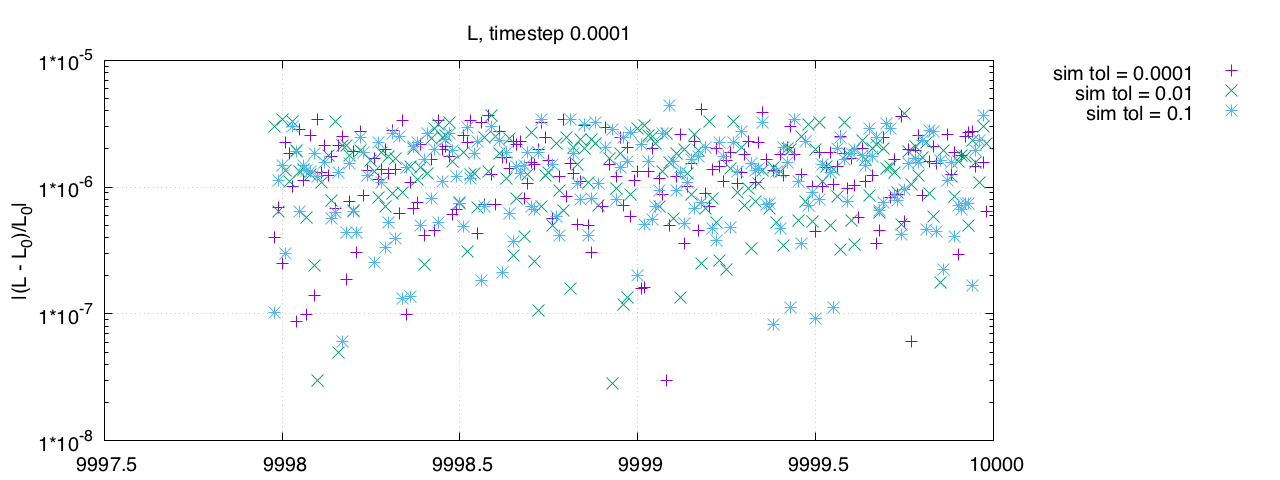
\includegraphics[width=\textwidth]
			{dt_0p0001_L_vs_sampleTime_endtime_1p0.png}}
		\caption{timestep $1 \times 10^{-4}$, $\frac{t}{T}$ from $998$ to $1000$}
	\end{subfigure}
	\vfill
	\begin{subfigure}[b]{0.49\textwidth}
		{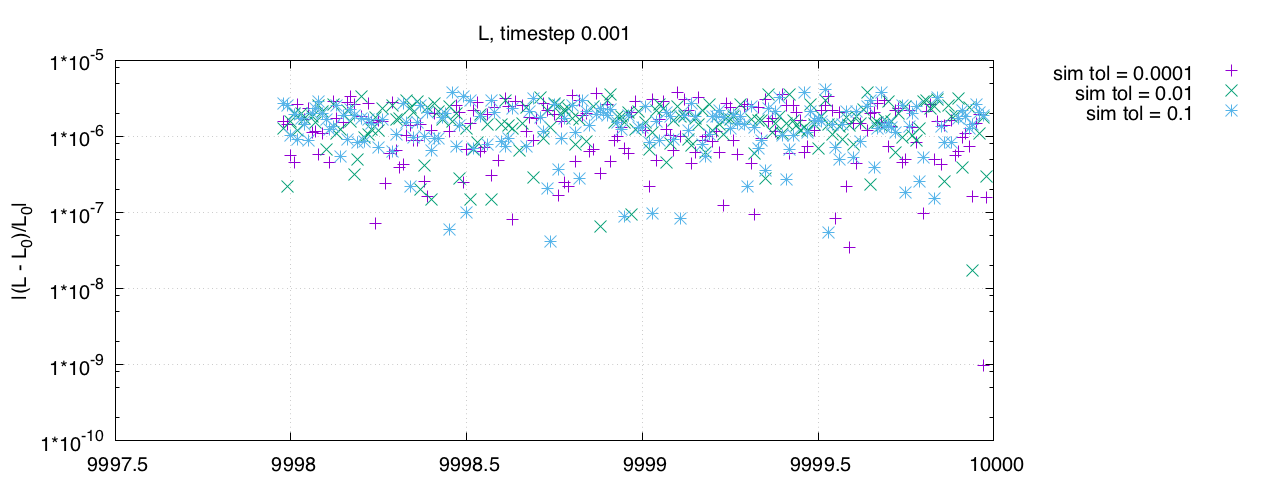
\includegraphics[width=\textwidth]
			{dt_0p001_L_vs_sampleTime_endtime_1p0.png}}
		\caption{timestep $1 \times 10^{-3}$, $\frac{t}{T}$ from $998$ to $1000$}
	\end{subfigure}
	\vfill
	\begin{subfigure}[b]{0.49\textwidth}
		{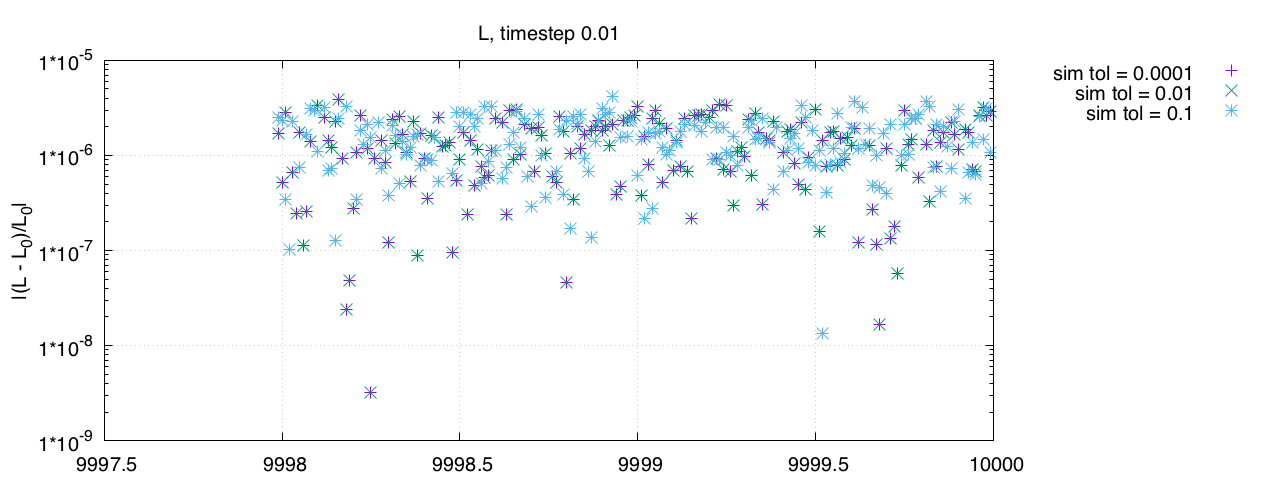
\includegraphics[width=\textwidth]
			{dt_0p01_L_vs_sampleTime_endtime_1p0.png}}
		\caption{timestep $1 \times 10^{-2}$, $\frac{t}{T}$ from $998$ to $1000$}
	\end{subfigure}
	\vfill
	\begin{subfigure}[b]{0.49\textwidth}
		{\includegraphics[width=\textwidth]
			{dt_0p1_L_vs_sampleTime_endtime_1p0.png}}
		\caption{timestep $1 \times 10^{-1}$, $\frac{t}{T}$ from $998$ to $1000$}
	\end{subfigure}
	\caption{\label{fig:res-labs} Angular momentum of the diatomic molecule, at various timesteps and at $\frac{t}{T} \in \left[ 9998, 10000\right]$ during the simulation. The two different tolerances in the $\textsf{RATTLE}$ algorithm were set equal.}
\end{figure}
%%%%%%%%%%%%%%%%%%%%%%%%%%%%%%%%%%%%%%%%%%%%%%%%%%%%